% This file was created with tikzplotlib v0.9.12.
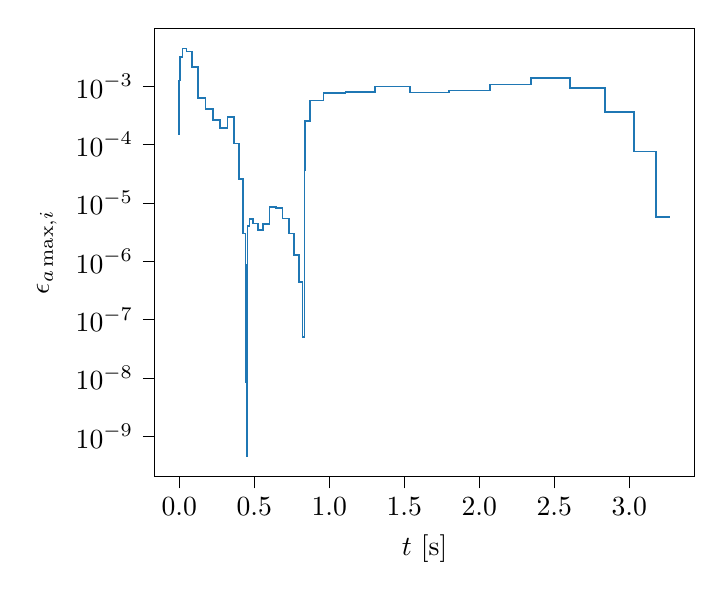
\begin{tikzpicture}

\definecolor{color0}{rgb}{0.12156862745098,0.466666666666667,0.705882352941177}

\begin{axis}[
log basis y={10},
tick align=outside,
tick pos=left,
x grid style={white!69.0196078431373!black},
xlabel={\(\displaystyle t\) [s]},
xmin=-0.163529513089662, xmax=3.4341197748829,
xtick style={color=black},
xtick={-0.5,0,0.5,1,1.5,2,2.5,3,3.5},
xticklabels={
  \(\displaystyle {\ensuremath{-}0.5}\),
  \(\displaystyle {0.0}\),
  \(\displaystyle {0.5}\),
  \(\displaystyle {1.0}\),
  \(\displaystyle {1.5}\),
  \(\displaystyle {2.0}\),
  \(\displaystyle {2.5}\),
  \(\displaystyle {3.0}\),
  \(\displaystyle {3.5}\)
},
y grid style={white!69.0196078431373!black},
ylabel={\(\displaystyle \epsilon_{a\max,i}\)},
ymin=2.04046103935055e-10, ymax=0.00979648154993535,
ymode=log,
ytick style={color=black},
ytick={1e-11,1e-10,1e-09,1e-08,1e-07,1e-06,1e-05,0.0001,0.001,0.01,0.1},
yticklabels={
  \(\displaystyle {10^{-11}}\),
  \(\displaystyle {10^{-10}}\),
  \(\displaystyle {10^{-9}}\),
  \(\displaystyle {10^{-8}}\),
  \(\displaystyle {10^{-7}}\),
  \(\displaystyle {10^{-6}}\),
  \(\displaystyle {10^{-5}}\),
  \(\displaystyle {10^{-4}}\),
  \(\displaystyle {10^{-3}}\),
  \(\displaystyle {10^{-2}}\),
  \(\displaystyle {10^{-1}}\)
}
]
\addplot [semithick, color0, const plot mark right]
table {%
0 0.000146994992838868
0.0056120056173798 0.00125292289388725
0.0221666130741685 0.00314387249522351
0.0488337052264625 0.0043844813195612
0.0842760827216659 0.00393434481218719
0.12671651675769 0.00209873568515404
0.174026866756148 0.000621985038014015
0.223834794217301 0.000403096267016022
0.273642721678455 0.000265571904107171
0.320953071676913 0.00019378641010478
0.363393505712937 0.000291872117247476
0.39883588320814 0.000104027295161562
0.425502975360434 2.58958219664476e-05
0.442057582817223 2.98590581696969e-06
0.447669588434603 8.41189278132351e-09
0.447669588434603 8.41189278132351e-09
0.447694744492815 1.8359842817035e-08
0.447768951264519 7.5999391554061e-08
0.447888487688025 2.41468485959326e-08
0.448047359718729 1.88759166772341e-08
0.448237600848921 1.75207278097712e-08
0.448449671593784 1.42346391259343e-08
0.448672937840577 1.53354383596719e-08
0.44889620408737 1.52805220810071e-08
0.449108274832234 1.06438581950435e-08
0.449298515962425 1.03126707633951e-08
0.44945738799313 6.64842918983019e-09
0.449576924416636 6.88261356635615e-09
0.44965113118834 4.55911143609573e-10
0.449676287246552 8.26349834069365e-08
0.449676287246552 8.26349834069365e-08
0.454574962603674 8.51797784523003e-07
0.469025348637549 4.02332336615575e-06
0.492302842652881 5.33599719521025e-06
0.523240213901389 4.4446898130187e-06
0.560286133405463 3.4613693394539e-06
0.60158296407088 4.2817599757961e-06
0.645059910367528 8.57511763484359e-06
0.688536856664177 8.11780238816371e-06
0.729833687329594 5.36976228832033e-06
0.766879606833668 2.9672842839517e-06
0.797816978082176 1.28705945318835e-06
0.821094472097507 4.43135741677917e-07
0.835544858131383 5.05669002370504e-08
0.840443533488505 3.68511837591641e-05
0.840443533488505 3.68511837591641e-05
0.87129471129975 0.000254332948352362
0.962301237854726 0.000568900175932206
1.10889966590181 0.000763222727881582
1.30373893811699 0.000787336791892987
1.53704899981345 0.000983035278810892
1.79713071027977 0.00077510766536352
2.0709424865465 0.00083638142077063
2.34475426281323 0.0010699943509009
2.60483597327954 0.00138563056811056
2.838146034976 0.000934379976011115
3.03298530719118 0.000362755353102018
3.17958373523827 7.5423030314595e-05
3.27059026179324 5.65795086222889e-06
};
\end{axis}

\end{tikzpicture}
